\documentclass[a2paper, 12pt]{article}
\usepackage[font={huge, bf}]{caption}
\usepackage{fontspec}
\setmainfont{Arial}
\usepackage{subcaption}
\usepackage{graphicx}
\usepackage{tikz}
\usepackage{tikzsymbols}
\usetikzlibrary{calc,patterns,shapes.geometric}
\usepackage{float}
\usepackage{pdflscape}
\usepackage{geometry}
\geometry{landscape, margin=2cm}
\captionsetup[subfigure]{justification=justified,singlelinecheck=false}
\pagestyle{empty}

\def\centerarc[#1](#2)(#3:#4:#5){\draw[#1] ($(#2)+({#5*cos(#3)},{#5*sin(#3)})$) arc (#3:#4:#5);}

\begin{document}
	\vspace*{\fill}
	\begin{figure}[!htbp]
		\centering
		\begin{subfigure}[b]{0.48\textwidth}
			\caption{Figure 1}
			\centering
			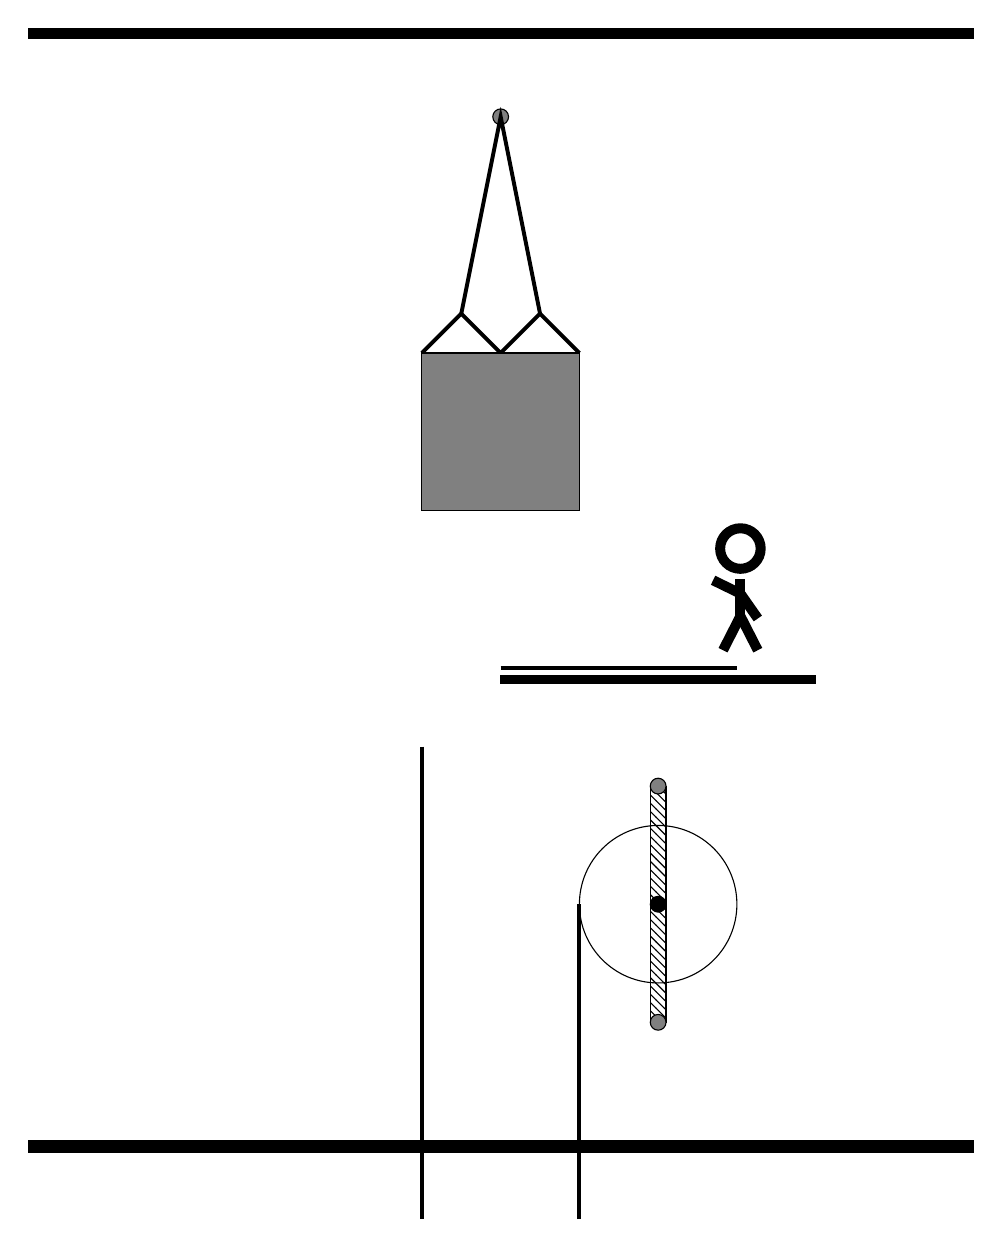
\begin{tikzpicture}
				\draw[fill=black] (-4, 14) rectangle (8, 14.125);
				
				\draw (4,3) circle (1);
				\draw[fill=black] (4,3) circle (0.1);
				\draw[pattern=north west lines, pattern color=black] (3.9,4.5) rectangle (4.1,1.5);
				\draw[fill=black!50] (4,4.5) circle (0.1);
				\draw[fill=black!50] (4,1.5) circle (0.1);
				
				\draw[fill=black!50] (2,13) circle (0.1);
				\draw[line width=0.5mm](1.5,10.5) -- (2,13) --  (2.5,10.5);
				\draw[line width=0.5mm](1,10) --  (1.5,10.5) -- (2,10) -- (2.5,10.5) -- (3,10);
				\draw[fill=black!50] (1, 10) rectangle (3, 8);
				
				\draw[line width = 0.5mm] (2,6) -- (5,6);
				\centerarc[line width = 0.5mm](2,5)(90:180:1);
				\draw[line width = 0.5mm] (1,5) -- (1,-1);
				\centerarc[line width = 0.5mm](2,-1)(180:360:1);
				\draw[line width = 0.5mm] (3,-1) -- (3,3);
				
				\node at (5, 7) {\scriptsize \Strichmaxerl[10][125][154]};
				\draw[fill=black] (2, 5.9) rectangle (6, 5.8);
				
				\draw[fill=black] (-4, 0) rectangle (8, -0.15);
			\end{tikzpicture}
		\end{subfigure}
		\hfill
		\begin{subfigure}[b]{0.48\textwidth}
			\caption{Figure 2}
			\centering
			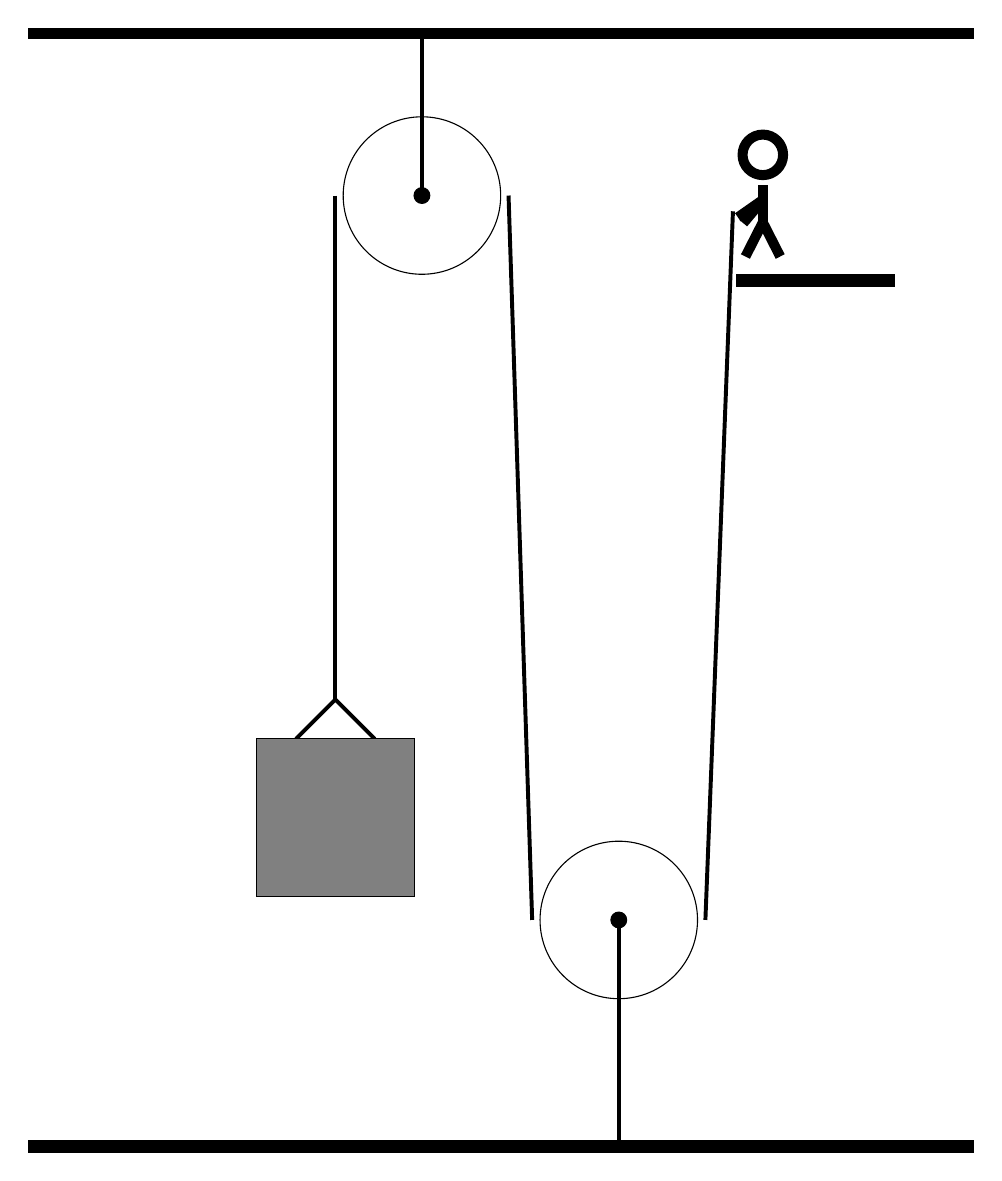
\begin{tikzpicture}
				\draw[fill=black] (-4, 14) rectangle (8, 14.125);
				
				\draw (3.5, 2.8) circle (1);
				\draw[fill=black] (3.5, 2.8) circle (0.1);
				\draw[line width=0.5mm] (3.5, 2.8) -- (3.5, 0);
				
				\draw (1, 12) circle (1);
				\draw[fill=black] (1, 12) circle (0.1);
				\draw[line width=0.5mm] (1, 14) -- (1, 12);
				
				\draw[line width=0.5mm](-0.6, 5.1) --  (-0.1, 5.6) -- (0.4, 5.1);
				\draw[fill=black!50] (-1.1, 5.1) rectangle (0.9, 3.1);
				
				\draw[line width=0.5mm](-0.1, 12) -- (-0.1, 5.6);
				\centerarc[line width=0.5mm](1, 12)(180:0:1.1)
				\draw[line width=0.5mm](2.1, 12) -- (2.4, 2.8);
				\centerarc[line width=0.5mm](3.5, 2.8)(180:360:1.1)
				\draw[line width=0.5mm](4.6, 2.8) -- (4.95, 11.8);
				
				\node at (5.3, 12) {\scriptsize \Strichmaxerl[10][35][-130]};
				\draw[fill=black] (5, 11) rectangle (7, 10.85);
				
				\draw[fill=black] (-4, 0) rectangle (8, -0.15);
			\end{tikzpicture}
		\end{subfigure}
	\end{figure}
		\vspace*{\fill}
\end{document}